% -*- latex -*-
%-----------------------------------------------------------------------
%;  Copyright (C) 2006
%;  Associated Universities, Inc. Washington DC, USA.
%;
%;  This program is free software; you can redistribute it and/or
%;  modify it under the terms of the GNU General Public License as
%;  published by the Free Software Foundation; either version 2 of
%;  the License, or (at your option) any later version.
%;
%;  This program is distributed in the hope that it will be useful,
%;  but WITHOUT ANY WARRANTY; without even the implied warranty of
%;  MERCHANTABILITY or FITNESS FOR A PARTICULAR PURPOSE.  See the
%;  GNU General Public License for more details.
%;
%;  You should have received a copy of the GNU General Public
%;  License along with this program; if not, write to the Free
%;  Software Foundation, Inc., 675 Massachusetts Ave, Cambridge,
%;  MA 02139, USA.
%;
%;  Correspondence concerning AIPS should be addressed as follows:
%;          Internet email: aipsmail@nrao.edu.
%;          Postal address: AIPS Project Office
%;                          National Radio Astronomy Observatory
%;                          520 Edgemont Road
%;                          Charlottesville, VA 22903-2475 USA
%-----------------------------------------------------------------------
%Body of final AIPSletter for 31 December 2005

\documentclass[twoside]{article}
\usepackage{graphics}

\newcommand{\AIPRELEASE}{December 31, 2005}
\newcommand{\AIPVOLUME}{Volume XXV}
\newcommand{\AIPNUMBER}{Number 2}
\newcommand{\RELEASENAME}{{\tt 31DEC05}}
\newcommand{\OLDNAME}{{\tt 31DEC04}}
\newcommand{\NEWNAME}{{\tt 31DEC06}}

%macros and title page format for the \AIPS\ letter.
\input LET98.MAC

\newcommand{\MYSpace}{-11pt}

\normalstyle

\section{General developments in \AIPS}

\subsection{Current and future releases}

We now have formal \AIPS\ releases on an annual basis.  Beginning very
recently, we offer a full binary installation method for both the
frozen and development versions  for MacIntosh OS/X, Solaris, and
Linux.  All architectures can do a full installation from the source
files.  The current release is called \RELEASENAME\ and is now frozen.
If you took a development copy of this version at some earlier date,
you may use the ``Midnight Job'' (MNJ) to bring it up to date.  You
need to run a MNJ only once in 2006 to convert your copy of
\RELEASENAME\ into the now frozen version.  When patches to 2005 are
announced, you may apply them with the MNJ\@.  This \Aipsletter\ is
intended to advise you of developments in this release.

We have begun a new version, called \NEWNAME, which is now under
development by the \AIPS\ Group.  You may fetch and install
a complete copy of this version at any time.  Having fetched \NEWNAME,
you may update your installation whenever you want by running the MNJ
which uses transaction files to copy and compile the code selectively
based on the code changes and compilations we have done.  We expect
users to take their source-only or binary version of \NEWNAME\ \AIPS\
over the Internet (via \emph{anonymous} ftp).  Both versions require
you to copy the installation procedure {\tt install.pl} via {\tt ftp};
the source-only version also requires you to copy the 70-Mbyte
{\tt 31DEC05.tar.gz} compressed tar file.

From {\tt mnj.aoc.nrao.edu}, the MNJ will serve up \AIPS\
incrementally --- or as a whole --- using the Unix tool {\tt cvs}
running with anonymous ftp.  Binary MNJs also use the {\tt rsync}
tool.  Linux sites will almost certainly have {\tt cvs} installed;
other sites may have installed it along with other GNU tools.
Secondary MNJs will still be possible using {\tt ssh} or {\tt rcp} or
NFS as with previous releases.  We have found that {\tt cvs} works
very well, although it has one quirk.  If a site modifies a file
locally but in an \AIPS-standard directory, {\tt cvs} will detect
the modification and attempt to reconcile the local version with the
NRAO-supplied version.  This usually produces a file that will not
compile or run as intended.
%\vfill\eject

\AIPS\ is now copyright \copyright\ 1995 through 2006 by Associated
Universities, Inc., NRAO's parent corporation, but may be made freely
available under the terms of the Free Software Foundation's General
Public License (GPL)\@.  This means that User Agreements are no longer
required, that \AIPS\ may be obtained via anonymous ftp without
contacting NRAO, and that the software may be redistributed (and/or
modified), under certain conditions.  The full text of the GPL can be
found in the \texttt{15JUL95} \Aipsletter\ and is included with every
distribution in file {\tt \$AIPS\_ROOT/{\it release-name}/COPYING}\@.

\subsection{Installing a new version}

If compiling locally, new releases must be installed from the tar ball
for that release.  If using the binary installation, a full new
installation must also be done with {\tt rsync}.  The {\tt cvs} system
requires this.  When installing a new \AIPS\ release in a system that
already has a previous release, we recommend that {\tt install.pl} be
used and that the previous release be left in place, at least until
the installation has been seen to work.  If you do this, then you will
not have to re-edit the disk, printer, and tape lists and can simply
skip all those pages in the {\tt install.pl} menus.  The old {\tt
  \$HOME/.AIPSRC} file may be left in place, but it will need to be
edited.  The lines giving the {\tt DOWNLOADED} and {\tt UNPACKED}
parameters should be deleted and the {\tt CCOMOPT} line should be
changed to point to the current release rather than the previous one
--- the {\tt -I} parameter really should be {\tt -I\$INC} but that
seems to confuse {\tt install.pl}.  Therefore, for now, the {\tt
  \$INC} has to be given in its full path name, which forces a re-edit
with each release.  If you have made special versions of {\tt
  UPDCONFIG} and {\tt do\_daily.{\it host}}, you should preserve them
under new names and restore them after the install.  If you have an
odd set of \AIPS\ versions, the {\tt \$AIPS\_ROOT/AIPSPATH.*SH} files
may need to be edited after the install to set the desired versions.

For Linux, Solaris Ultra, and MacIntosh systems, a binary installation
is available from CDrom, supported by {\tt install.pl}.  Alternatively,
the frozen version may be installed with the binary installation
method now present in {\tt install.pl}.  The ftp site for downloading
files directly has been eliminated.

%\vfill\eject

\section{Binary installations and updates}

GNU has provided compilers for the \AIPS\ community at no cost for
many years.  While remarkably good, these compilers have suffered from
both minor errors and from their generality.  When some vendor sets
out to make a compiler for a very specific architecture, it is
possible --- not guaranteed --- to create a compiler that produces
binaries that run faster than those produced by GNU's {\tt g77}.
Unfortunately, these vendors have to recover their costs in producing
these compilers and so may charge for them at a rate that is difficult
or prohibitive for many \AIPS\ users.  Such is the case with IBM's {\tt
  xlf} compiler for PPC chips, including the MacIntosh OS/X systems,
for SUN's SUNWspro compiler suite, and for Intel's {\tt ifort}
compiler.   These compilers produce executables that run about 50\%\
faster (30\%\ faster for Intel) than those produced by {\tt g77} on
these operating systems and cpus.  Fortunately, their licensing
agreements allow us to ship executables to our users along with the
required run-time libraries.  The binaries produced by the Intel
compiler are quite large because they contain optimizations for modern
PIV cpus, older PIV cpus, and for general computers such as AMDs.  The
specific optimizations to be used are selected at run time.

The code to implement the binary installation and binary updates via
the MNJ is comparatively simple.  Every night, a {\tt cron} job run on
the master \AIPS\ machine in Socorro, does the necessary magic to make
the daily cvs snapshot of \AIPS, builds the tar-ball, orders the three
architectures at the AOC to do ordinary text MNJs, and then {\tt
  rsync}'s the binaries and text to a special area on the computer
used for public {\tt ftp} access to NRAO in Socorro.  The installation
script must be fetched from the AOC anonymous ftp area to your desired
{\tt \$AIPS\_ROOT} area and then executed with

\begin{center}
\vskip -12pt
{\tt \Large perl install.pl -n}
\vskip -12pt
\end{center}

With the {\tt -n} option, the script will skip fetching and unpacking
the tar-ball and the compiler queries and usage.  It does a variety of
{\tt rsync} commands to fetch a complete copy of the \AIPS\ version
including libraries and all executables.  It marks the installation as
a binary one by creating a special 0-byte file in {\tt \$SYSLOCAL}\@.
The MNJ then detects this file and replaces the compile steps with
{\tt rsync} operations on the binary areas.  The {\tt cvs} utility is
still used for updating the source code and other text areas.

There are some limitations with binary installations.  The AP size
will be 20 Megabytes which is a good size for most machines and
problems, but too small for the largest-memory computers and biggest
problems.  Furthermore, without a matching compiler, it will be
difficult to develop any local programs as additions to the standard
\AIPS\ package.

\section{Improvements of interest to users in \RELEASENAME}

We expect to continue publishing the  \Aipsletter\ approximately every
six months along with the annual releases.  There have been a number
of changes in \RELEASENAME\@.  In the last six months, we have
developed new tasks {\tt CLCOP} to copy {\tt CL} table data between
IFs, {\tt REAMP} to rescale fluxes in uv data, {\tt SPIXR} to fit
spectral indices to image cubes, and {\tt CCRES} to remove and restore
Clean components from images.  Two new {\tt VLBAUTIL} procedures were
written to download from the web and apply to VLBI data measurements
of the  ionosphere and earth orientation.  A service program {\tt
  REUSE} was written to convert public catalog \AIPS\ installations to
user-private installations.  The new verb {\tt QINP} allows users to
resume looking at {\tt INPUTS} at the last page they were examining.
\NEWNAME\ already has a change in {\tt UVCON} to model interferometers
which have position-dependent primary beam patterns.  This change was
judged too significant to put into nearly frozen code.

{\tt 31DEC04} and \RELEASENAME\ use a new numbering scheme for
magnetic tape logical unit numbers that is incompatible with previous
versions.  Thus all tape tasks and the server {\tt TPMON} must be from
one of these two releases.  Other than this, \RELEASENAME\ is
compatible in all major ways with the with the {\tt 15OCT98} and later
releases.  There are significant incompatibilities with older versions.

\subsection{UV data calibration}

\subsubsection{Calibrator models}

In the {\tt 30JUN04} edition of the \AIPSLETTER\ we announced the
availability of VLA flux calibrator models for the 3 highest frequency
bands observed with the VLA in \AIPS\@.  Here we announce the
availability of flux calibrator models at all bands from K through L
for 3C48 and 3C286, in addition to the models at K, Q and U for 3C138
and 3C147.  Models for 3C138 and 3C147 at the lower frequencies should
become available over the next year.  To see what models are available
in \AIPS\ type {\tt CALDIR}; to load a model use the task {\tt CALRD}.

Now that most VLA primary flux calibrators have models, their use
should be the default way to obtain amplitude calibration for the
VLA\@.  See the \AIPS\ \Cookbook\ for details.  The VLA primary flux
calibrators are resolved at most frequencies and configurations.  Even
in the configurations and frequencies where they are not resolved
(\eg\ L band in D array) there are many confusing sources, so in {\it
all situations} a model will make the flux calibration more accurate.
Note that multiple facets were required to image the calibrators and
confusing sources at the lower frequencies.  We have found, however,
that the Clean components from the exterior facets may be included in
the {\tt CC} table of the primary facet with no loss of accuracy in
calibration.  When using the models, there is no need to limit the
$uv$ range or antennas in {\tt CALIB}, making automated data reduction
even easier.

When working with the calibrator models, we discovered a serious
problem with the way models are computed from images.  In order to
handle coordinate rotation, the central pixel and the reference pixel
of the image are both relevant to model phase computation.  Before mid
November 2005, \AIPS\ had no mechanism to retain the central pixel
information when images are changed in size, \eg\ by {\tt SUBIM}\@.
All calibrator models were corrected on November 1, 2005 to have their
central pixel be the original central pixel even though the images
have been reduced significantly in size.  Prior to that date, the
calibrator models would get the correct amplitude calibration but
would introduce a position shift into the phases.  Fortunately, the
primary amplitude calibrators are rarely if ever used to to provide
phases for the target sources.

\subsubsection{The VLBA and the Earth Orientation Parameters}

When VLBI data are correlated, the position of the Earth's North pole
and the offset between Earth rotation time and clock time must be
known.  Unfortunately, these parameters must be calculated using
measurements taken on the day in question, so the best estimates are
not determined for several weeks after the fact.  Given the cost of
VLBI recording media, the data must be correlated using predicted EOPs
rather than the final, good estimates.  Compounding this basic
problem, it was found recently that the VLBA correlator had a
systematic error in selecting the Earth Orientation Parameters (EOP)
estimate it used, causing a very preliminary estimate to be used from
May 2003 to August 2005. Fortunately, the parameters that were used
are recorded in the previously unused {\tt CT} table.  {\tt FITLD} was
revised to handle this table more carefully and to add to it
information on the $uv$-data time range to which each entry applies.

The task {\tt CLCOR} was given a new {\tt OPCODE='EOPS'} to read a
text file containing the latest EOP parameters and to correct phases
for any differences between them and the parameters used at
correlation.  A  procedure called {\tt VLBAEOPS} was added to the {\tt
  VLBAUTIL} {\tt RUN} file.  It can fetch the latest EOP data from the
USNO over the web and then use them in {\tt CLCOR}\@.  This correction
should be run on all VLBA data that require accurate phases,
particularly phase-reference observations.  For details see VLBA Test
Memo 69 by R. C. Walker, V. Dhawan, W. Brisken, J. Benson, L. Kogan,
and J. Romney from {\tt http://www.vlba.nrao.edu/memos/test/}.

\subsubsection{Other VLBI changes}

In addition to {\tt VLBAEOPS} mentioned above, a number of other
changes were made to the {\tt VLBAUTIL} {\tt RUN} package.  New
procedure {\tt VLBATECR} downloads the electron content data from the
web that applies to the data set and then runs {\tt TECOR}\@.  These
two procedures make clever use of the {\tt SYSTEM} verb to fetch and
apply information from the web.  Procedure {\tt VLBALOAD} now allows
data to be taken from disk and {\tt VLBAMPCL} defends itself against a
common form of user input.

{\tt SNSMO} is the task recommended for smoothing VLBI solutions since
it does a better job of handling delays and rates with their effects
on phase.  However, {\tt SNSMO} adopted the heavy-handed assumption
that all rates should be the same and so averaged all polarizations
and IFs producing identical output rates.  This was changed to have
{\tt SMOTYPE 'VLBI'} average over polarization to avoid changing
apparent instrumental polarization, but to keep IFs separate.  A new
{\tt SMOTYPE 'VLRI'} was added to retain the previous averaging over
IFs.

{\tt FITLD} was changed to recognize that a station named ``Y'' with a
sensitivity of 1.0 is actually the phased VLA\@.  In that case, the
recorded $T_{\rm sys}$ is actually $T_{\rm sys} / T_{\rm ant}$, a fact
that is signaled by setting the antenna temperature to $-1.0$ in the
{\tt TY} table.  Prior to this correction, very wrong amplitude
calibrations would be found for the phased VLA\@.  Errors corrected in
{\tt FITLD} include a date comparison that could cause the task to
skip data files rather than loading them, uninitialized extension file
version numbers in numerous subroutine calls, and a rearrangement of
code to allow proper file management when trying to close down
gracefully after an error occurs.

\subsubsection{Other $uv$-data changes}

\begin{description}
\myitem{FLAGR} and {\tt FINDR} were changed to regard a failed
     solution (when finding antenna-based amplitudes, phases, weights)
     as grounds for deleting the data.  This simple fix seems to have
     made this into a quite useful flagging task using essentially
     only default adverb values.
\myitem{CLCOP} is a new task to copy the calibration for one
     polarization into that for the other.  It can swap them and even
     write a 2-polarization file from a 1-polarization input file.
\myitem{REAMP} is a new task to rescale amplitudes and weights.
\myitem{RESEQ} was completely rewritten to allow complicated antenna
     renumbering operations.
\myitem{FILLM} was changed to get the correct bandwidth for modes 8
     and 9 which is $50 / 2^8$ MHz.  The previous value (half as
     large) led to wrong reference channels, bandwidths, and other
     minor errors.
\myitem{CALIB} was changed to count ``failed'' solutions
     differently.  Previously, missing data were counted as failed
     which is more than a little confusing.
\myitem{CPASS} was changed to accept error returns from the fitting
     subroutines.  It will quit on one of the errors, but will write
     the solutions into the {\tt BP} table even when the fitting
     routines say they did not converge.  It is not clear that this
     task has ever worked.
\end{description}

\subsection{Imaging}

\subsubsection{Managing box files}

{\tt IMAGR} has a rather complicated set of adverbs plus {\tt BOXFILE}
options which may be used to define facets, resolutions, and Clean
boxes.  There are several tasks which have been written to help manage
these parameters, primarily the {\tt BOXFILE} content.  Initially,
these tasks were fairly simple but they have been changed to handle
most of the options that are used in {\tt IMAGR}\@.  {\tt BOXES} was
written to add Clean boxes to a {\tt BOXFILE} which defined the
facets, but with the addition of {\tt NFIELD}, {\tt RASHIFT}, and {\tt
DECSHIFT} the facets may be defined in other ways.  {\tt FIXBX} was
written to correct the boxes of one {\tt BOXFILE} which defined its
facets to those facets defined in another {\tt BOXFILE}\@.  But, with
the addition of {\tt NMAPS}, {\tt NOISE}, {\tt PBSIZE}, {\tt NBOXES},
{\tt CLBOX} and {\tt NGAUSS} to describe old imaging parameters (along
with {\tt INFILE}) and {\tt NFIELD}, {\tt RASHIFT}, and {\tt DECSHIFT}
to describe new imaging parameters *along with {\tt BOXFILE}) the
faceting may be described completely with adverbs.  {\tt CHKFC} was
initially written to test the {\tt BOXFILE} output of {\tt SETFC}, but
can now define the facets and boxes with {\tt NFIELD}, {\tt RASHIFT},
{\tt DECSHIFT}, {\tt NBOXES}, and {\tt CLBOX}\@.

\subsubsection{Miscellaneous matters}

\begin{description}
\myitem{CCRES} is a new task to add or subtract Clean components from
          an image.  Unlike RSTOR, there is no requirement that the
          components lie on cells or that the image be a power of 2 in
          size.
\myitem{RSTOR} was revised to subtract as well as add Clean components
          to an image.
\myitem{IMAGR} was corrected.  The user's {\tt MINPATCH} value was
          lost when cleaning a small window and not restored when next
          cleaning a large window.
\myitem{Single-dish} imaging was changed.  {\tt SELSD} and {\tt GRIDR}
          were removed along with the concept of ``projected''
          coordinates in the $uv$ location.  Galactic and Ecliptic as
          well as the usual celestial coordinates are now allowed in
          {\tt SDIMG}\@.  A path to import GBT data into \AIPS\ for
          imaging is available in Green Bank.
\end{description}

\subsection{Analysis}

\subsubsection{Spectral index}

With the development of the EVLA, interest in spectral-index issues
has grown.  {\tt IMMOD} was changed to allow the addition of up to
four model images per execution.  {\tt UVMOD} was changed to allow
different spectral-indices for each of the up to four model objects.
{\tt MCUBE} was changed to allow the user to force the creation of a
{\tt SEQ.NUM.} axis ignoring some axis coordinate that differs in an
irregular way.  This axis is called {\tt FQID} when the coordinate is
frequency and the values of the coordinate are stored in a {\tt FQ}
table attached to the output image cube.  The coordinates of any type
that are ignored on such an axis are stored in the history file.

A new task named {\tt SPIXR} was written.  It reads a transposed cube
(frequency axis first) and fits to it an image of spectral index and,
optionally, spectral index curvature using least squares.  Early
testing of this task indicates that issues of spatial resolution and
blanking will be important in its use.  It is intended to use the
output of {\tt SPIXR} as an optional input to {\tt IMAGR} to correct
for spectral index while doing bandwidth synthesis imaging of
continuum sources.

\subsubsection{Miscellaneous}

\begin{description}
\myitem{CCEDT} was overhauled so that its less known option of
          automatic box splitting might actually work.  Corrected
          handling of boxes for images of less common types.
\myitem{RMSD} was given the option to output the local mean value
          instead of the local rms.
\myitem{SAD} was given the option to read an image of the rms.
\end{description}

\subsection{Plotting}

\begin{description}
\myitem{TVCPS} was generalized to read one image from disk for each
           image plane that is visible.  This will allow large images
           to be written to the output PostScript file for
           hue-intensity and three-color displays.
\myitem{SNPLT} was corrected to select IFs correctly when plotting
       {\tt PC} tables.
\myitem{Point} plotting was further clarified, making a consistent set
        of symbols across all tasks using the standard list of
        available symbols.
\end{description}

\subsection{General items}

\begin{description}
\myitem{QINP} is a new verb.  It resumes the previous {\tt INP} or
       {\tt INPUTS} with the last page viewed.  Thus, after viewing a
       page and changing the adverbs on the page, the user may re-view
       that page without having to start back at page 1.
\myitem{SYSTEM} is a powerful verb that invokes a command to the
       operating system.  It was enhanced with additional adverbs to
       allow for very long commands.
\myitem{APROPO} will now include all task, verb, adverb, and procedure
       names as well as the words in the one-line comments of the help
       files
\end{description}

\subsubsection{Miscellaneous matters for programmer types}

\begin{description}
\myitem{Dynamic} memory now uses {\tt LONGINT} as the data type for
        the array offset parameter.  This translates to {\tt
        INTEGER*8} on 64-bit computers where it has been tested.
        The trick of using the pseudo-AP routines with dynamic memory
        will not work on some of these computers because the 1000s of
        variables which are pointers into the pseudo-AP have not been
        translated to {\tt LONGINT}s.
\myitem{REUSE} is a new service program.  It translates an \AIPS\
        system that was set up with public (multiple user) catalogs
        into a system with separate catalogs and files names for each
        user.  {\tt FILAIP} was changed to make the error of having
        public catalogs very unlikely.
\myitem{install.pl} was changed for the changes in {\tt FILAIP} and to
        recognize AMD 64s making corrections in {\tt FORTOPT} and in
        the {\tt XAS} {\tt Makefile}.
\end{description}

\subsection{D\ae mon mysteries}

Two mysteries have arisen affecting the \AIPS\ d\ae mons.  The first
affects the message and Tektronix servers.  They are run as programs
inside an {\tt xterm}.  At at least one site, we found that the
command has to be invoked as\\
\centerline{{\tt xterm -e '\$LOAD/MSGSRV.EXE ' \&}}\\
with quote marks and a blank character ahead of the close quote.  At
most sites, this grammar is apparently acceptable if not required.
But, at all Solaris and some Linux sites, this grammar causes the
command to fail.  Does anyone out there understand what is going on?

The second mystery concerns the performance of the \AIPS\ TV {\tt
XAS}\@.  Compared to RedHat 9 and previous systems, the performance
appears to be compromised under RedHat Enterprise.  It is acceptable,
but noticeably slower, using {\tt tv=local} Unix sockets.  Using Inet
sockets, the communication to {\tt XAS} appears to be very erratic,
with rapid response for short intervals followed by no response for
comparable intervals.  This occurs only when the computer is actually
looping back to itself; the communication between computers appears to
be as fast as ever.  Any suggestions?????

\vfill\eject

\section{Patch Distribution for \OLDNAME}

As before, important bug fixes and selected improvements in
\OLDNAME\ and \RELEASENAME\ can be downloaded via the Web beginning
at:

\begin{center}
\vskip -10pt
{\tt http://www.aoc.nrao.edu/aips/patch.html}
\vskip -10pt
\end{center}

Alternatively one can use {\it anonymous} \ftp\ to the NRAO server
{\tt ftp.aoc.nrao.edu}.  Documentation about patches to a release is
placed on this site at {\tt pub/software/aips/}{\it release-name} and
the code is placed in suitable subdirectories below this.  As bugs in
\NEWNAME\ are found, they are simply corrected since \NEWNAME\ remains
under development.  Corrections and additions are made with a midnight
job rather than with manual patches.

The patch system has changed because we now have binary installations.
We now actually patch the master copy of the frozen version.  This
means that a MNJ run on \OLDNAME\ after the patches listed below will
fetch the corrected code and/or binaries rather than failing.
Similarly, patches announced for \RELEASENAME\ during the next year
will be available via MNJ as well as {\tt ftp}.  Installations of
\OLDNAME\ and \RELEASENAME\ after the patch date will contain the
corrected code.

The \OLDNAME\ release is no longer available for installation.  It
had a few important patches most of which were released in April when
we changed the patch system.  For correcting existing \OLDNAME\
releases, the patches are:
\begin{enumerate}
\item\ {\tt OTFUV, OTFIN} to handle both byte orders of 12m OTF
      data {\it 2005-01-06}
\item\ {\tt CXPOLN} procedure, {\tt CXCLN} task need
      modern image names {\it 2005-04-22}
\item\ {\tt TVFLG} and {\tt SPFLG} required improved
      error handling and modern {\tt FLAGVER} default
      {\it 2005-04-22}
\item\ {\tt WIPER} function {\tt FLAG AREA} aborted on
      wrong button push {\it 2005-04-22}
\item\ {\tt FIXBX} could handle complicated cases but not simple
      ones {\it 2005-04-22}
\item\ {\tt POSSM} used wrong units in output text file
      {\it 2005-04-22}
\item\ {\tt CL2HF} aborts under Linux {\it 2005-04-22}
\item\ {\tt TCOPY} used wrong (old) tape LUNs {\it 2005-04-22}
\item\ {\tt BPASS} gets wrong solutions when channel 1 of of the
      first source was flagged {\it 2005-04-22}
\item\ {\tt BOXES} could handle complicated cases but not simple ones
      {\it 2005-08-16}
\item\ {\tt CALIB} looses track of the {\tt SN} table when writing a
      {\tt FG} table {\it 2005-08-16}
\item\ {\tt FITLD} wrongly concluded data were too early and did not
      handle cal transfer correctly for the phased VLA {\it 2005-08-16}
\end{enumerate}

\section{Recent \AIPS\ and related Memoranda}

The following new EVLA Memorandum is available from the NRAO web
pages ({\tt http://www.aoc.nrao.edu/evla/memolist.shtml})

\begin{tabular}{lp{5.8in}}
96 &Imaging at Wide Field of View for a Plane Array\\
   &Leonid Kogan \\
   &9/20/2005\\
   &We consider the array located at a plane. The coordinate system we
    chose has U, V axes at the array plane, and W axis perpendicular
    to the array plane. W components of the baselines are equal zero
    and therefore expressions describing the Fourier transform pairs:
    IMAGE $<->$ VISIBILITIES do not include the W component of the
    vector directed to the current point at the source. As a result
    this Fourier transform is becoming two dimensional at the whole
    semi sphere of the sky.  This is obviously true for a snapshot
    observation. The method to connect different time snapshot
    observations is given.
\end{tabular}

The following new VLBA Test Memorandum is available from the NRAO web
pages ({\tt http://www.vlba.nrao.edu/memos/test/})

\begin{tabular}{lp{5.8in}}
69&Inappropriate EOP on the VLBA Correlator\\
  &R. C. Walker, V. Dhawan, W. Brisken, J. Benson, L. Kogan, \&\ J.
   Romney \\
  &10/06/2005\\
  &A bug has been found in the job generator for the VLBA correlator
   that caused it to use predicted rather than measured Earth
   Orientation Parameters (EOP) between May 2003 and August 2005. The
   errors introduced often are sufficiently large to adversely affect
   phase referencing observations and other observations that rely on
   an accurate correlator model. The nature of the problem and its
   impact are discussed in this memo. Correcting data is
   straightforward using the new EOPS option in the AIPS task CLCOR.
   Users just wishing to make corrections without worrying about the
   gory details can consult Section 2, or simply follow the CLCOR help
   file. It has become apparent while dealing with this problem that
   even occasional projects from outside the time period of the bug
   have been correlated with poor EOP. Usually this is because their
   job scripts were prepared too close to the observe date. So any
   user depending on an accurate correlator model may wish to check
   their EOP.
\end{tabular}

\section{\AIPS\ Distribution}

We are now able to log apparent MNJ accesses, downloads of the tar
balls and {\tt rsync} accesses.  We count these by unique IP address.
Since dial-up connections may be assigned different IP addresses at
different times, this will be a bit of an over-estimate of actual
sites.  However, a single IP address is often used to provide \AIPS\
to a number of computers, so these numbers are probably an
under-estimate of the number of computers running current versions of
\AIPS\@.  We have abandoned the registration system as obsolete and
onerous.  In 2005, a total of 246 different IP addresses downloaded
the frozen form of \OLDNAME\ and 832 IP addresses downloaded
\RELEASENAME\ in tarball or binary form.  Fully 982 IP addresses
accessed the NRAO cvs master.  Each of these has at least installed
\RELEASENAME\ and 252 appear to have run the MNJ on \RELEASENAME\ at
least occasionally.  The total number of unique IP addresses in these
three lists was 1460.  48 sites accessed \OLDNAME\ in binary form,
while 299 sites used the binary form of \RELEASENAME\@.  The attached
figure shows the cumulative number of unique sites, cvs access sites,
tar-ball/binary download sites and binary access sites known to us as
a function of week in 2005.

\centerline{\resizebox{3.8in}{!}{\includegraphics{FIG/PLOTIT5b.PS}}}

Since the registration system, always under-utilized, has now been
abandoned, we are left with analysis by IP address.  The table below
lists the IP addresses for 2005 by the final qualifier for shipments
of the {\tt 31DEC05} tarball, the {\tt 31DEC04} tarball, and access to
the cvs site.  The numbers in the cvs column include those sites that
install {\tt 31DEC05}, run a midnight job for {\tt 31DEC05}, or
run a final ``catch-up'' MNJ for {\tt 31DEC04}\@.  The comments come
from what appears to be a semi-official list of Internet codes.
Sorting is on the ``unique'' column, which counts unique IP addresses
over the other three columns:
\vfill\eject

\vspace{10pt}
\begin{center}
\begin{tabular}{lrrrrl}
\hline\hline
Code  & {\tt 31DEC04} & {\tt 31DEC05} & cvs site & unique & Comments \\
\hline
edu     &   55 &  199 &  283 &  382 &  US Educational \\
net     &   14 &   68 &   90 &  131 &  Network \\
uk      &   11 &   58 &   51 &   82 &  United Kingdom \\
jp      &   20 &   50 &   44 &   78 &  Japan \\
com     &    9 &   32 &   34 &   54 &  US Commercial \\
org     &    1 &   10 &   52 &   54 &  Non-Profit Organization \\
au      &    7 &   28 &   26 &   46 &  Australia \\
es      &    1 &   33 &   37 &   45 &  Spain \\
it      &    5 &   21 &   13 &   33 &  Italy \\
de      &    4 &   17 &   18 &   31 &  Germany \\
ca      &    4 &   18 &   19 &   29 &  Canada \\
gov     &    8 &   13 &   20 &   27 &  US Government \\
mil     &    5 &   17 &   13 &   22 &  US Military \\
pl      &    2 &   13 &    9 &   18 &  Poland \\
in      &    6 &   10 &    7 &   16 &  India \\
nl      &    4 &    8 &    9 &   14 &  Netherlands \\
fr      &    3 &   10 &    2 &   14 &  France \\
tw      &    6 &    7 &    7 &   10 &  Taiwan \\
cn      &    3 &    4 &    3 &    8 &  China \\
br      &    3 &    4 &    1 &    7 &  Brazil \\
kr      &    2 &    5 &    5 &    7 &  Korea (South) \\
mx      &    2 &    6 &    5 &    6 &  Mexico \\
pt      &    2 &    4 &    3 &    5 &  Portugal \\
ru      &    1 &    3 &    2 &    5 &  Russian Federation \\
inva    &    0 &    0 &    5 &    5 &  (Germany, key invalid)\\
se      &    1 &    2 &    1 &    4 &  Sweden \\
ar      &    1 &    2 &    2 &    4 &  Argentina \\
fi      &    0 &    3 &    4 &    4 &  Finland \\
ie      &    0 &    4 &    4 &    4 &  Ireland \\
cl      &    1 &    1 &    1 &    3 &  Chile \\
be      &    1 &    0 &    2 &    3 &  Belgium \\
il      &    0 &    3 &    1 &    3 &  Israel \\
za      &    0 &    1 &    3 &    3 &  South Africa \\
ch      &    1 &    0 &    1 &    2 &  Switzerland \\
at      &    2 &    0 &    0 &    2 &  Austria \\
hu      &    1 &    2 &    0 &    2 &  Hungary \\
dk      &    0 &    2 &    2 &    2 &  Denmark \\
co      &    0 &    2 &    0 &    2 &  Colombia \\
th      &    0 &    2 &    0 &    2 &  Thailand \\
cz      &    0 &    1 &    0 &    1 &  Czech Republic \\
yu      &    0 &    1 &    0 &    1 &  Yugoslavia \\
id      &    0 &    1 &    0 &    1 &  Indonesia \\
gr      &    0 &    1 &    1 &    1 &  Greece \\
mu      &    0 &    1 &    0 &    1 &  Mauritius \\
hr      &    0 &    1 &    0 &    1 &  Croatia (Hrvatska) \\
sk      &    0 &    1 &    0 &    1 &  Slovak Republic \\
None    &    1 &    7 &   13 &   14 &   \\
Unknown &   59 &  156 &  189 &  270 &   \\
 \hline
Total   &  246 &  832 &  982 & 1460 &   \\
 \hline
\end{tabular}
\end{center}

%\section{\AIPS\ Order Form}

%Conscientious readers will note that this issue does not contain a
%copy of the \AIPS\ Order Form.  Ernie Allen, who processes these
%forms, does not remember any of the paper forms being submitted this
%century.  Henceforth,
%To submit a request for a CD copy of \AIPS\
%or paper copies of documentation, see\\
%\centerline{{\tt http://www.aoc.nrao.edu/aips/forms/aipsorder.shtml}}\\
%or contact us at {\tt daip@nrao.edu}.

\vfill\eject

% Order form and mailer page
%\cleardoublepage
\pagestyle{empty}
%\vfill
%\centerline{\resizebox{!}{23.3cm}{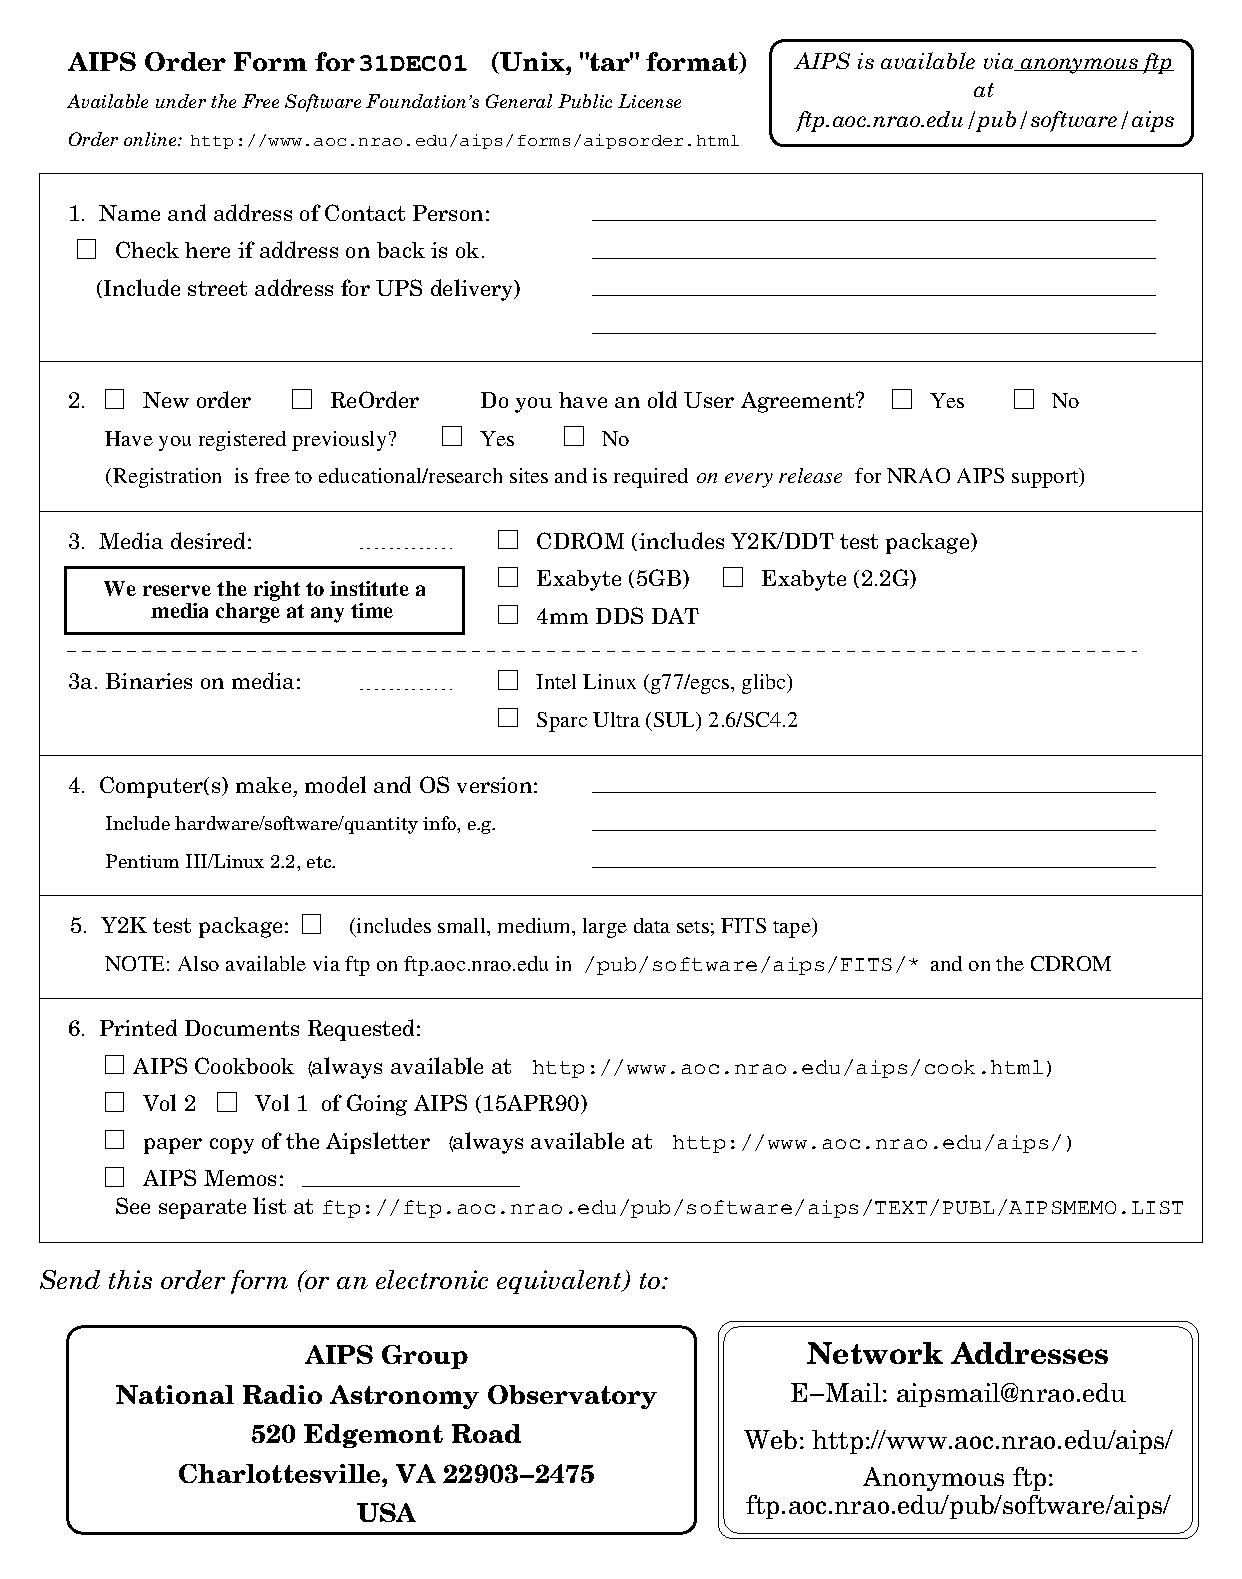
\includegraphics{FIG/AIPSORDER.PS}}}
%\vfill\eject
\vbox to 4.4in{
\vspace{12pt}
%\centerline{\rotatebox{-90}{\resizebox{!}{3.5in}{%
%\includegraphics{FIG/Mandrill.color.plt}}}}
\centerline{\resizebox{!}{3.5in}{\includegraphics{FIG/Mandrill.eps}}}
\vspace{12pt}
\centerline{{\huge \tt \AIPRELEASE}}
\vspace{12pt}
\vfill}
\phantom{...}
\centerline{\resizebox{!}{!}{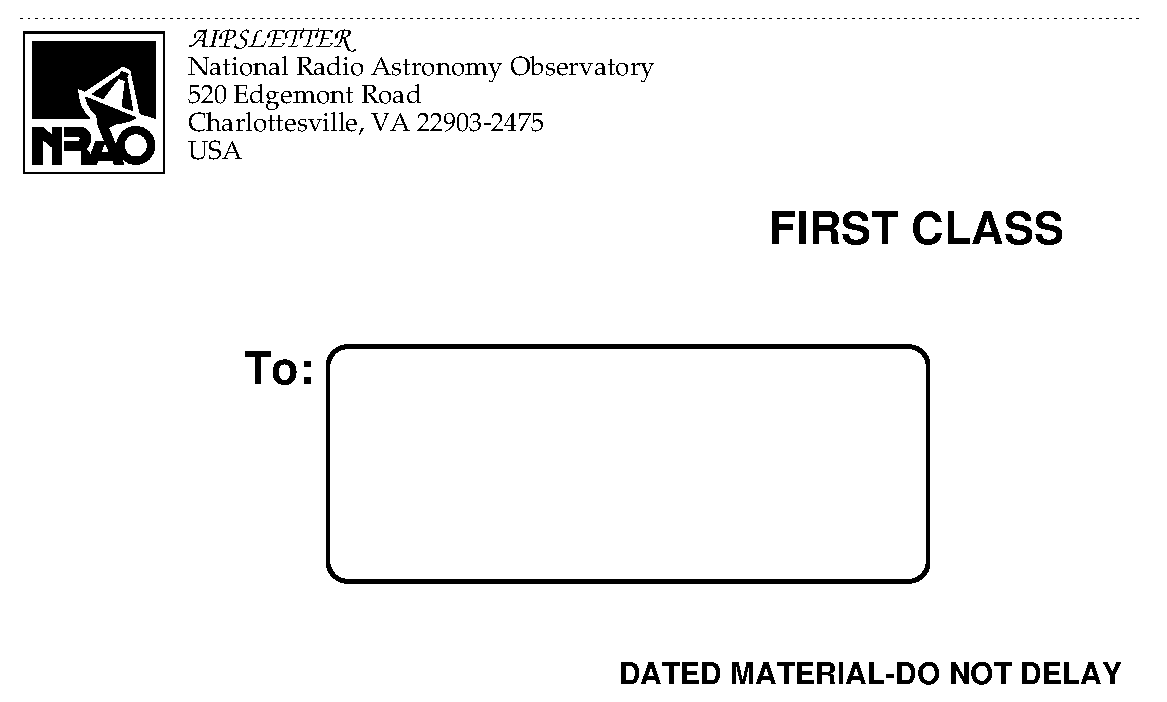
\includegraphics{FIG/AIPSLETM.PS}}}

\end{document}
